\documentclass{article}
\usepackage[utf8]{inputenc}
\usepackage{graphicx}
\usepackage{listings}
\usepackage[dvipsnames]{xcolor}
\usepackage{amsmath}
\usepackage{hyperref}
\usepackage{geometry}
 \geometry{
 a4paper,
 total={170mm,257mm},
 left=20mm,
 top=20mm,
 }
\newcommand{\sectionlinetwo}[2]{%
  \nointerlineskip \vspace{.5\baselineskip}\hspace{\fill}
  {\color{#1}
    \resizebox{0.5\linewidth}{2ex}
    {{%
    {\begin{tikzpicture}
    \node  (C) at (0,0) {};
    \node (D) at (9,0) {};
    \path (C) to [ornament=#2] (D);
    \end{tikzpicture}}}}}%
    \hspace{\fill}
    \par\nointerlineskip \vspace{.5\baselineskip}
  }
\definecolor{azure}{rgb}{0.0, 0.5, 1.0}
\definecolor{forestgreen}{rgb}{0.13, 0.55, 0.13}
\definecolor{codegreen}{rgb}{0,0.6,0}
\definecolor{codegray}{rgb}{0.5,0.5,0.5}
\definecolor{codepurple}{rgb}{0.58,0,0.82}
\definecolor{backcolour}{rgb}{0.95,0.95,0.92}

\lstdefinestyle{mystyle}{
    backgroundcolor=\color{backcolour},   
    commentstyle=\color{codegreen},
    keywordstyle=\color{magenta},
    numberstyle=\tiny\color{codegray},
    stringstyle=\color{codepurple},
    basicstyle=\ttfamily\footnotesize,
    breakatwhitespace=false,         
    breaklines=true,                 
    captionpos=b,                    
    keepspaces=true,                 
    numbers=left,                    
    numbersep=5pt,                  
    showspaces=false,                
    showstringspaces=false,
    showtabs=false,                  
    tabsize=2
}
\lstset{style=mystyle}

\title{Submission for HW 3 (Programming Assignment)\\\small{\textit{CS 427: Mathematics for Data Science, Autumn 2020-21}}}
\author{K. Sai Anuroop, 170030035}
\date{\today}

\begin{document}

\maketitle

\begin{flushleft}
\section{Question 1}
Plot a 3D graph and a contour map of $f(x,y)=x^2-y^2\ \forall\ x,y\in[-5,5]$
\begin{figure}[htp]
        \centering
        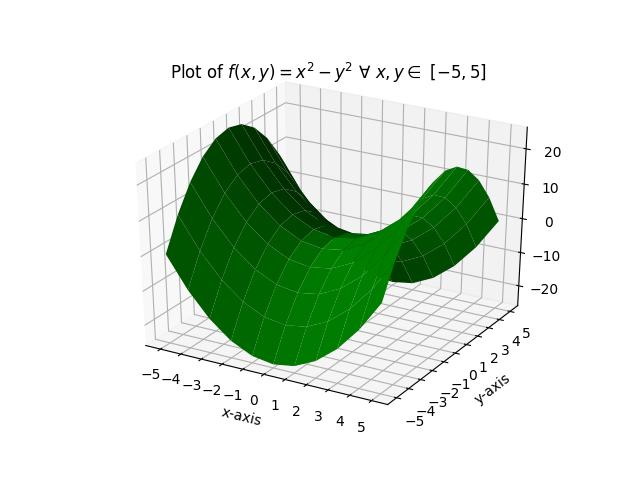
\includegraphics[width=9cm]{x2y2_saddle_surface.png}\\
        \caption{3D graph}
\end{figure}
\begin{figure}[htp]
        \centering
        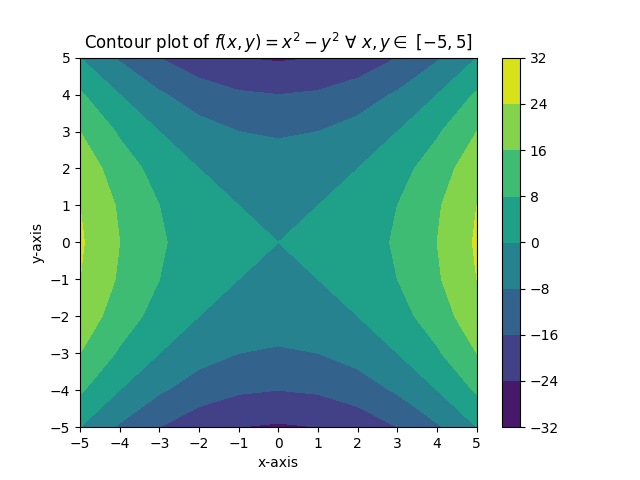
\includegraphics[width=9cm]{x2y2_saddle_contour.png}\\
        \caption{Contour map}
\end{figure}
\clearpage
\section{Question 2}
Randomly generate a set of $24$ points that belong to the set $\{(x,y):x,y\in[-5,5]$. Create a scatter plot and outline the convex hull of the set you just created.
\begin{figure}[htp]
        \centering
        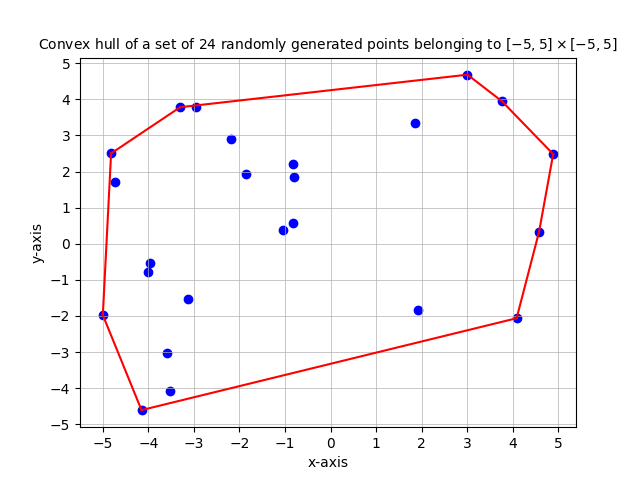
\includegraphics[width=9cm]{conv_hull.png}\\
        \caption{Scatter plot and convex hull}
\end{figure}
\section{Question 3}
Check if the function $f(x)=x^{T}Ax$ for $A\in R^{2\times2}$ where all components of $x$ are integers in $[-10,10]$, is convex. Find $11$ counter examples if it is not.\\~\\

I take a random vector $x$ where $x_{ij}\in[-10,10]$ for $i,j=\{1,2\}$. I then rotate and scale it using the matrix $A:=\Big(\begin{matrix}\cos\theta & \sin\theta \\ \sin\theta & \cos\theta\end{matrix}\Big)$. Here $f(x)=x^{T}Ax=(x^{2}+y^{2})\cos\theta+2xy\sin\theta$. There is a result which states that $f(x)=x^{T}Ax$ is convex if and only if $A$ is positive semidefinite. By the way I defined the matrix $A$, it is symmetric. However, it can be analysed that for some values of $\theta$, $f$ takes negative values. So I provide $11$ such values of $A$ for which $f$ is not convex. For better visualisation, I plotted the rotated and scaled vector $Ax$ for some values of $A$. I also plot the corresponding surfaces of $f$.\\
Here are the counter-examples in terms of the matrix $A$:\\
$\Big(\begin{matrix}0.27 & 0.96 \\ 0.96 & 0.27\end{matrix}\Big)$
$\Big(\begin{matrix}0.17 & 0.99 \\ 0.99 & 0.17\end{matrix}\Big)$
$\Big(\begin{matrix}0.07 & 1.0 \\ 1.0 & 0.07\end{matrix}\Big)$
$\Big(\begin{matrix}-0.03 & 1.0 \\ 1.0 & -0.03\end{matrix}\Big)$
$\Big(\begin{matrix}-0.13 & 0.99 \\ 0.99 & -0.13\end{matrix}\Big)$
$\Big(\begin{matrix}-0.23 & 0.97 \\ 0.97 & -0.23\end{matrix}\Big)$
$\Big(\begin{matrix}-0.32 & 0.95 \\ 0.95 & -0.32\end{matrix}\Big)$
$\Big(\begin{matrix}-0.42 & 0.91 \\ 0.91 & -0.42\end{matrix}\Big)$
$\Big(\begin{matrix}-0.5 & 0.86 \\ 0.86 & -0.5\end{matrix}\Big)$
$\Big(\begin{matrix}-0.59 & 0.81 \\ -0.59 & 0.81\end{matrix}\Big)$
$\Big(\begin{matrix}-0.67 & 0.75 \\ 0.75 & -0.67\end{matrix}\Big)$\\
Clearly as seen in the below plots, $f$ loses its convexity as we vary the value of $\theta$ from $0$ to $\pi$.\\
\begin{figure}[htp]
        \centering
        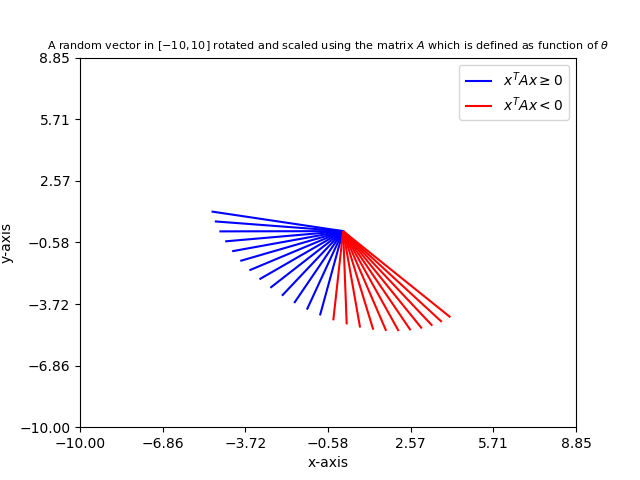
\includegraphics[width=9cm]{psd.png}\\
        \caption{Rotated and scaled vectors $Ax$ for different matrices $A$}
\end{figure}
\begin{figure}[htp]
        \centering
        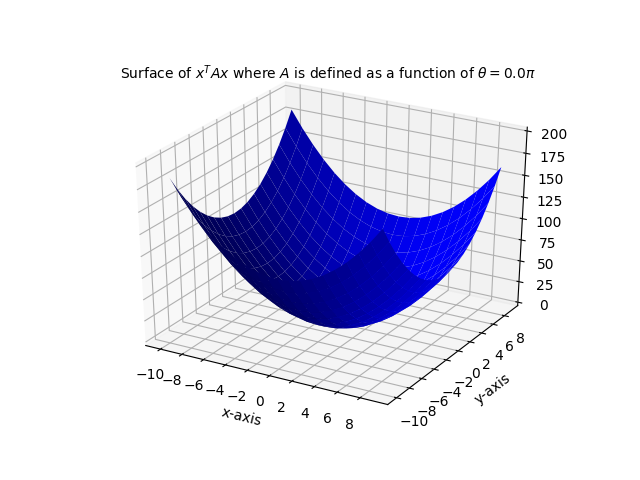
\includegraphics[width=9cm]{0pi.png}\\
        \caption{Surface of $f$ for $\theta=0$}
\end{figure}
\begin{figure}[htp]
        \centering
        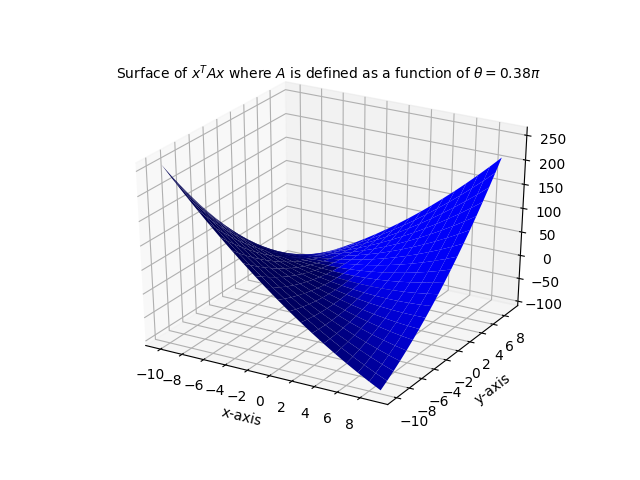
\includegraphics[width=9cm]{38pi.png}\\
        \caption{Surface of $f$ for $\theta=0.38\pi$}
\end{figure}
\begin{figure}[htp]
        \centering
        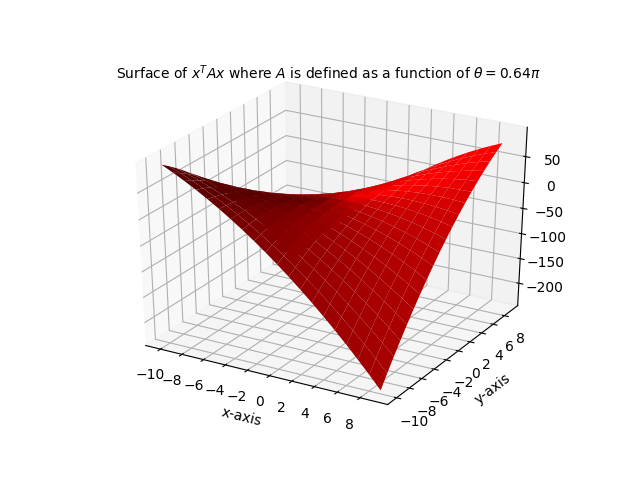
\includegraphics[width=9cm]{64pi.png}\\
        \caption{Surface of $f$ for $\theta=0.64\pi$}
\end{figure}
\begin{figure}[htp]
        \centering
        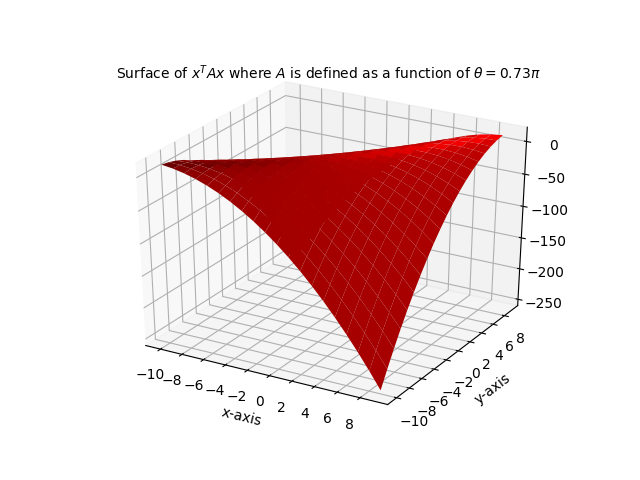
\includegraphics[width=9cm]{73pi.png}\\
        \caption{Surface of $f$ for $\theta=0.73\pi$}
\end{figure}
\clearpage
\begin{figure}[htp]
        \centering
        
\includegraphics[width=9cm]{qr-code.png}\\
        Scan this QR code to access the GitHub repository of my homweork solutions at \href{https://github.com/ksanu1998/MDS_HW_Solutions}{https://github.com/ksanu1998/MDS\_HW\_Solutions}
\end{figure}
\end{flushleft}
\end{document}
